\chapter{Various Special Structures in \LaTeX{}}

\paragraph{Introduction}
This chapter presents different special environments in \LaTeX{} apart from the display math mode and verbatim form previously, such as lists, figures, tables, and minipages.

\section{Lists}

\subsection{Unordered Lists}

\paragraph{itemize}
The ability to organize things into a \textit{list} is essential in any documenting system. In \LaTeX{}, we can achieve this by using the \verb|itemize| environment with the \texttt{\textbackslash item} command. For example, if we write
\begin{lstlisting}
\begin{itemize}
\item Canada
\item Japan \begin{itemize}
    \item Tokyo
    \item Kyoto
    \end{itemize}
\item Korea \begin{itemize}
    \item Seoul
    \item Pusan
    \end{itemize}
\end{itemize}  
\end{lstlisting}
then it will show up as
\begin{itemize}
\item Canada
\item Japan \begin{itemize}
    \item Tokyo
    \item Kyoto
    \end{itemize}
\item Korea \begin{itemize}
    \item Seoul
    \item Pusan
    \end{itemize}
\end{itemize}  
Notice that the list can be nested and the items are \textit{unordered/bulleted}.

\subsection{Ordered Lists}

\paragraph{enumerate}
Similarly, we can have an \textit{ordered/numbered} list by using the \verb|enumerate| environment. For example, by typing
\begin{lstlisting}
\begin{enumerate}
    \item A robot may not injure a human being ... % (continue)
    \item A robot must obey the orders given it by human ...
    \item A robot must protect its own existence ...
\end{enumerate}    
\end{lstlisting}
we acquire the following outcome:
\begin{enumerate}
    \item A robot may not injure a human being or, through inaction, allow a human being to come to harm.
    \item A robot must obey the orders given it by human beings except where such orders would conflict with the First Law.
    \item A robot must protect its own existence as long as such protection does not conflict with the First or Second Law.
\end{enumerate}
It is also possible to have nested \verb|enumerate| groups.

\paragraph{enumitem}
The \verb|enumitem| package enhances the typesetting of lists. One of the prime utilities is to change the starting labels or bullets for every item by providing the \verb|label| option. For example,
\begin{lstlisting}
\begin{enumerate}[label=\alph*)]
    \item Apple
    \item Banana
    \item Grape
\end{enumerate}
\end{lstlisting}
generates
\begin{enumerate}[label=\alph*)]
    \item Apple
    \item Banana
    \item Grape
\end{enumerate}
There are other possible choices for \verb|label|, e.g. \texttt{\textbackslash arabic*}, \texttt{\textbackslash roman*}, \texttt{\textbackslash Roman*}, \texttt{\textbackslash Alph*}. Another usage of the \verb|enumitem| package is to make a continued list. For example, by ticking the \verb|resume*| option:
\begin{lstlisting}
\begin{enumerate}[resume*]
    \item Watermelon
    \item Orange
\end{enumerate}    
\end{lstlisting}
we have
\begin{enumerate}[resume*]
    \item Watermelon
    \item Orange
\end{enumerate}

\section{Figures and Tables}

\subsection{Figures}

\paragraph{figure, includegraphics}
To import figures into the document, we need to load the \verb|graphics| package and then use the \texttt{\textbackslash includegraphics\{<file\_name>\}} command. Given that the image is placed under the project directory, we hereby go through an example which is displayed as Figure \ref{fig:ada} on the next page. The code to produce that figure is
\begin{lstlisting}
\begin{figure}[ht!]
\centering
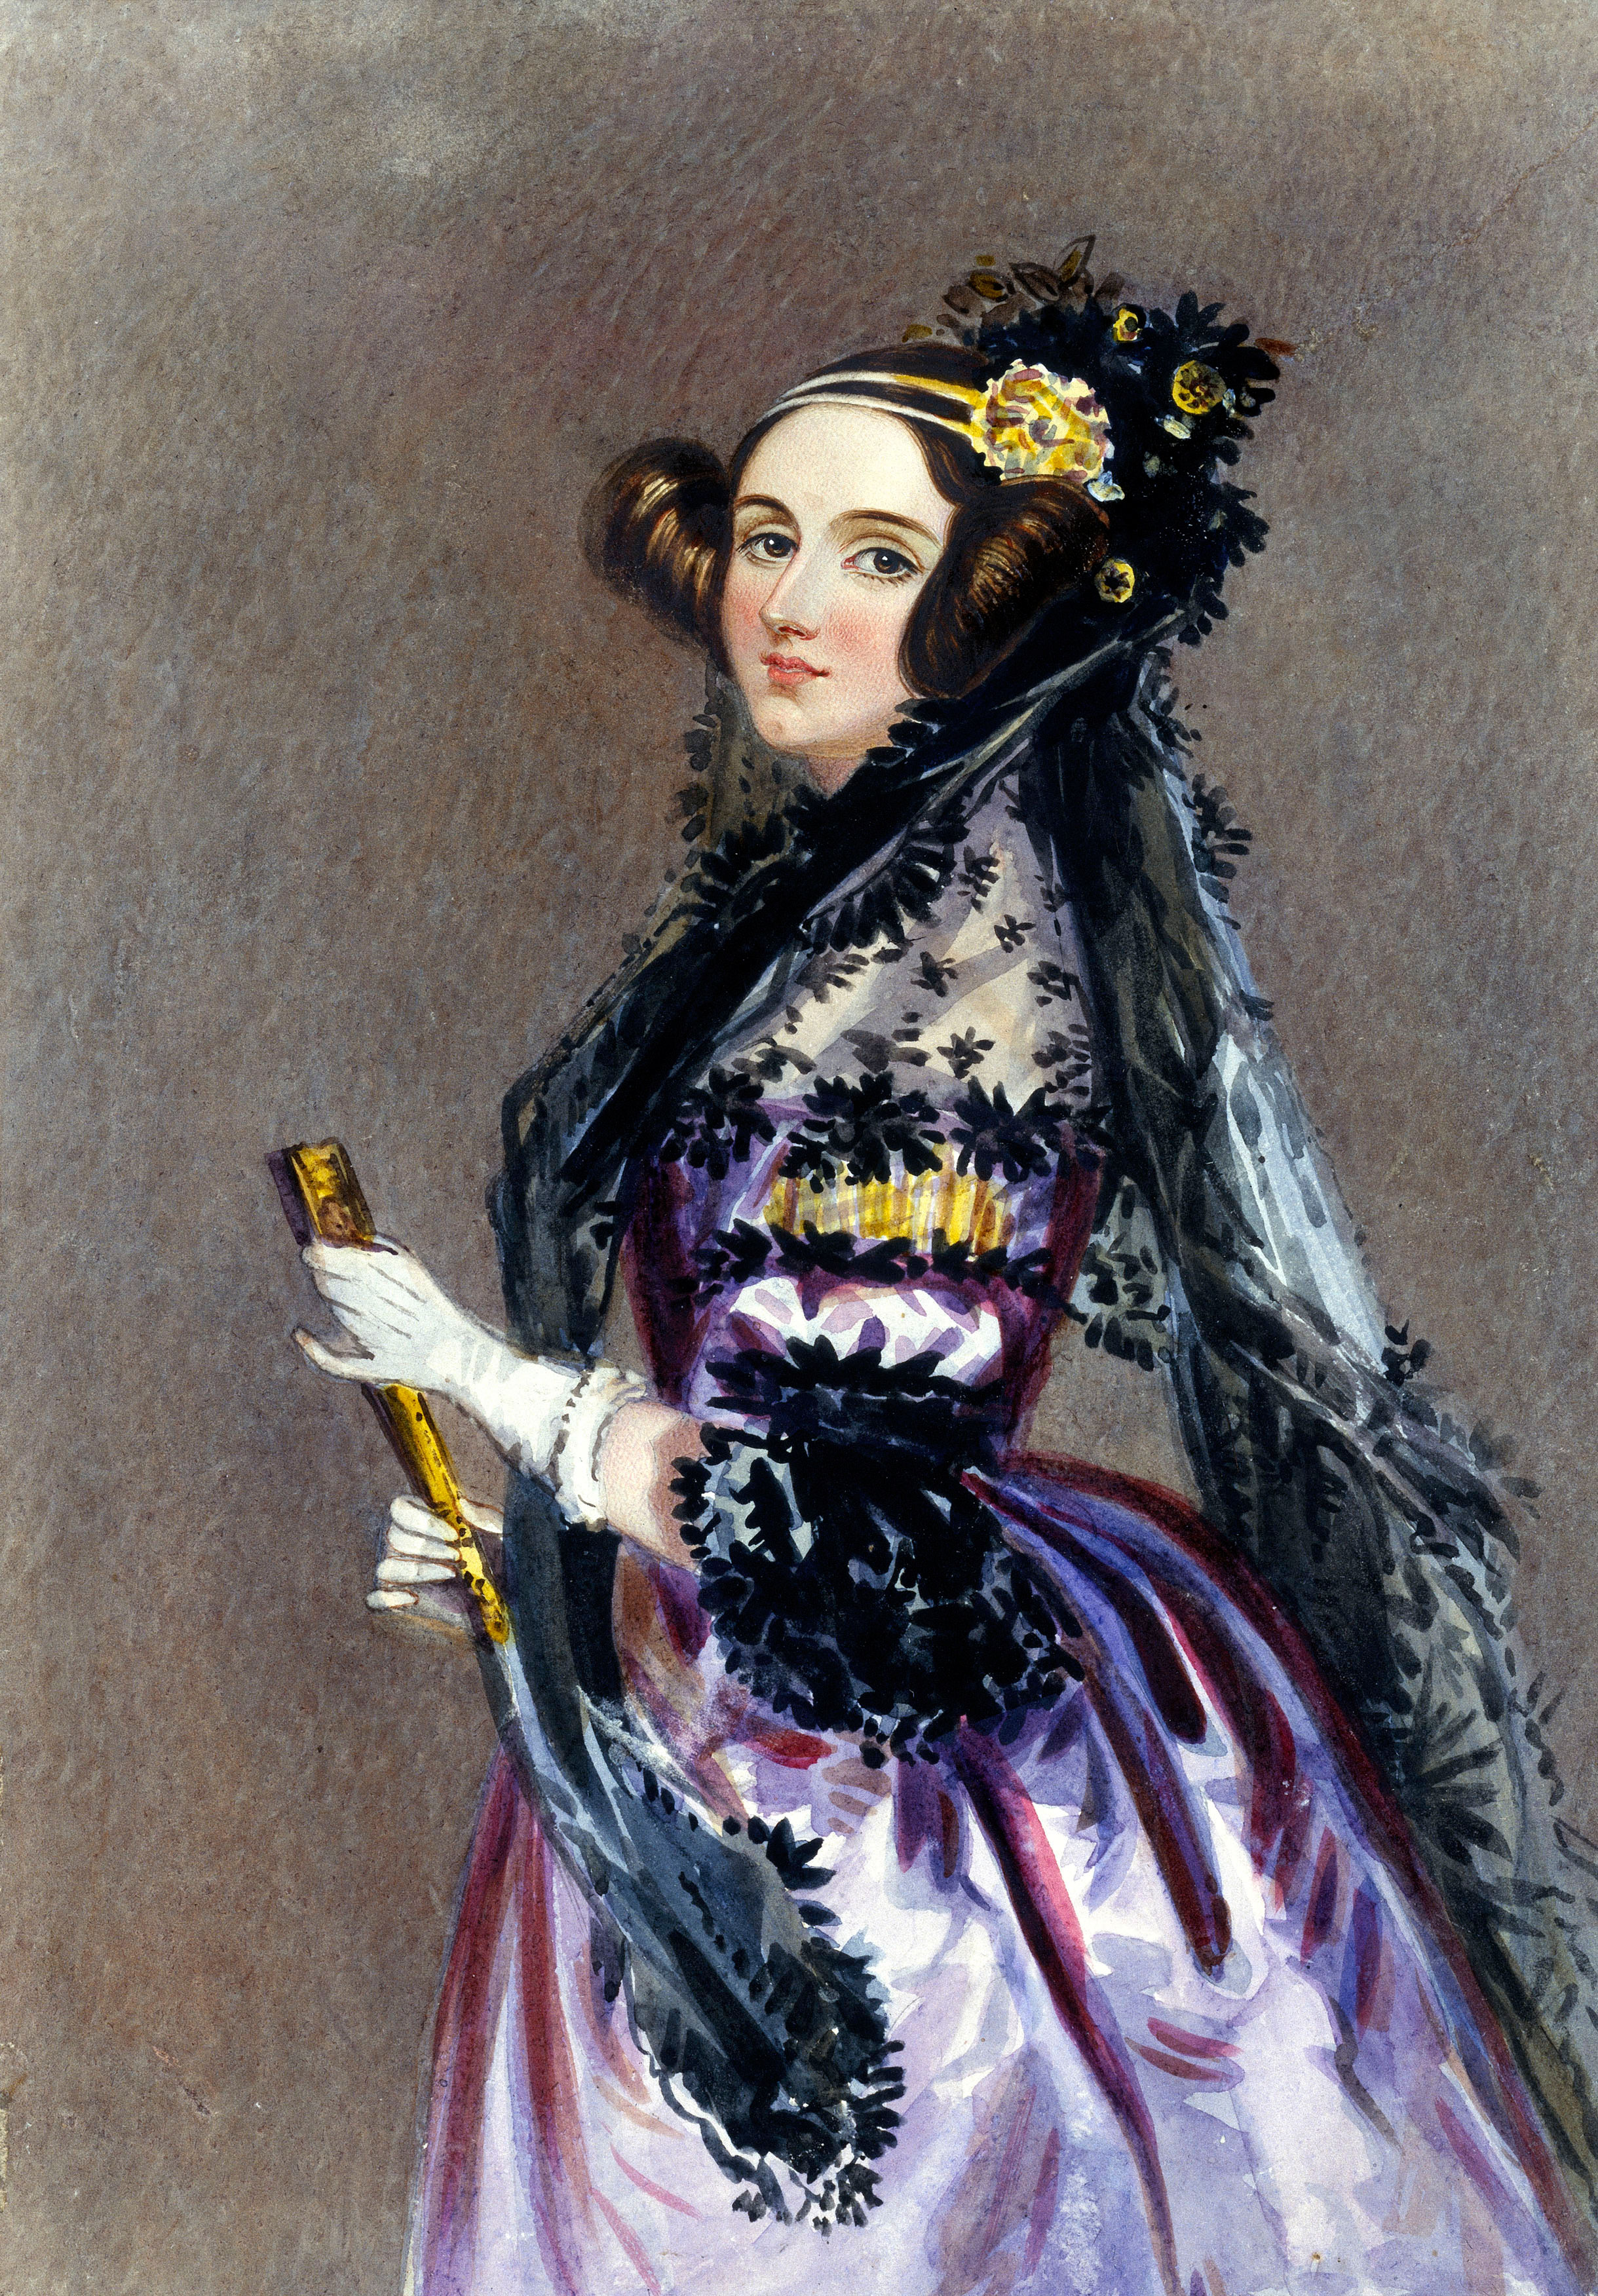
\includegraphics[width=0.4\linewidth]{graphics/Ada_Lovelace_portrait.jpg} % replace the path with your own file
\caption{The portrait of Ada Lovelace.}
\label{fig:ada}
\end{figure}    
\end{lstlisting}
\begin{figure}[ht!]
\centering
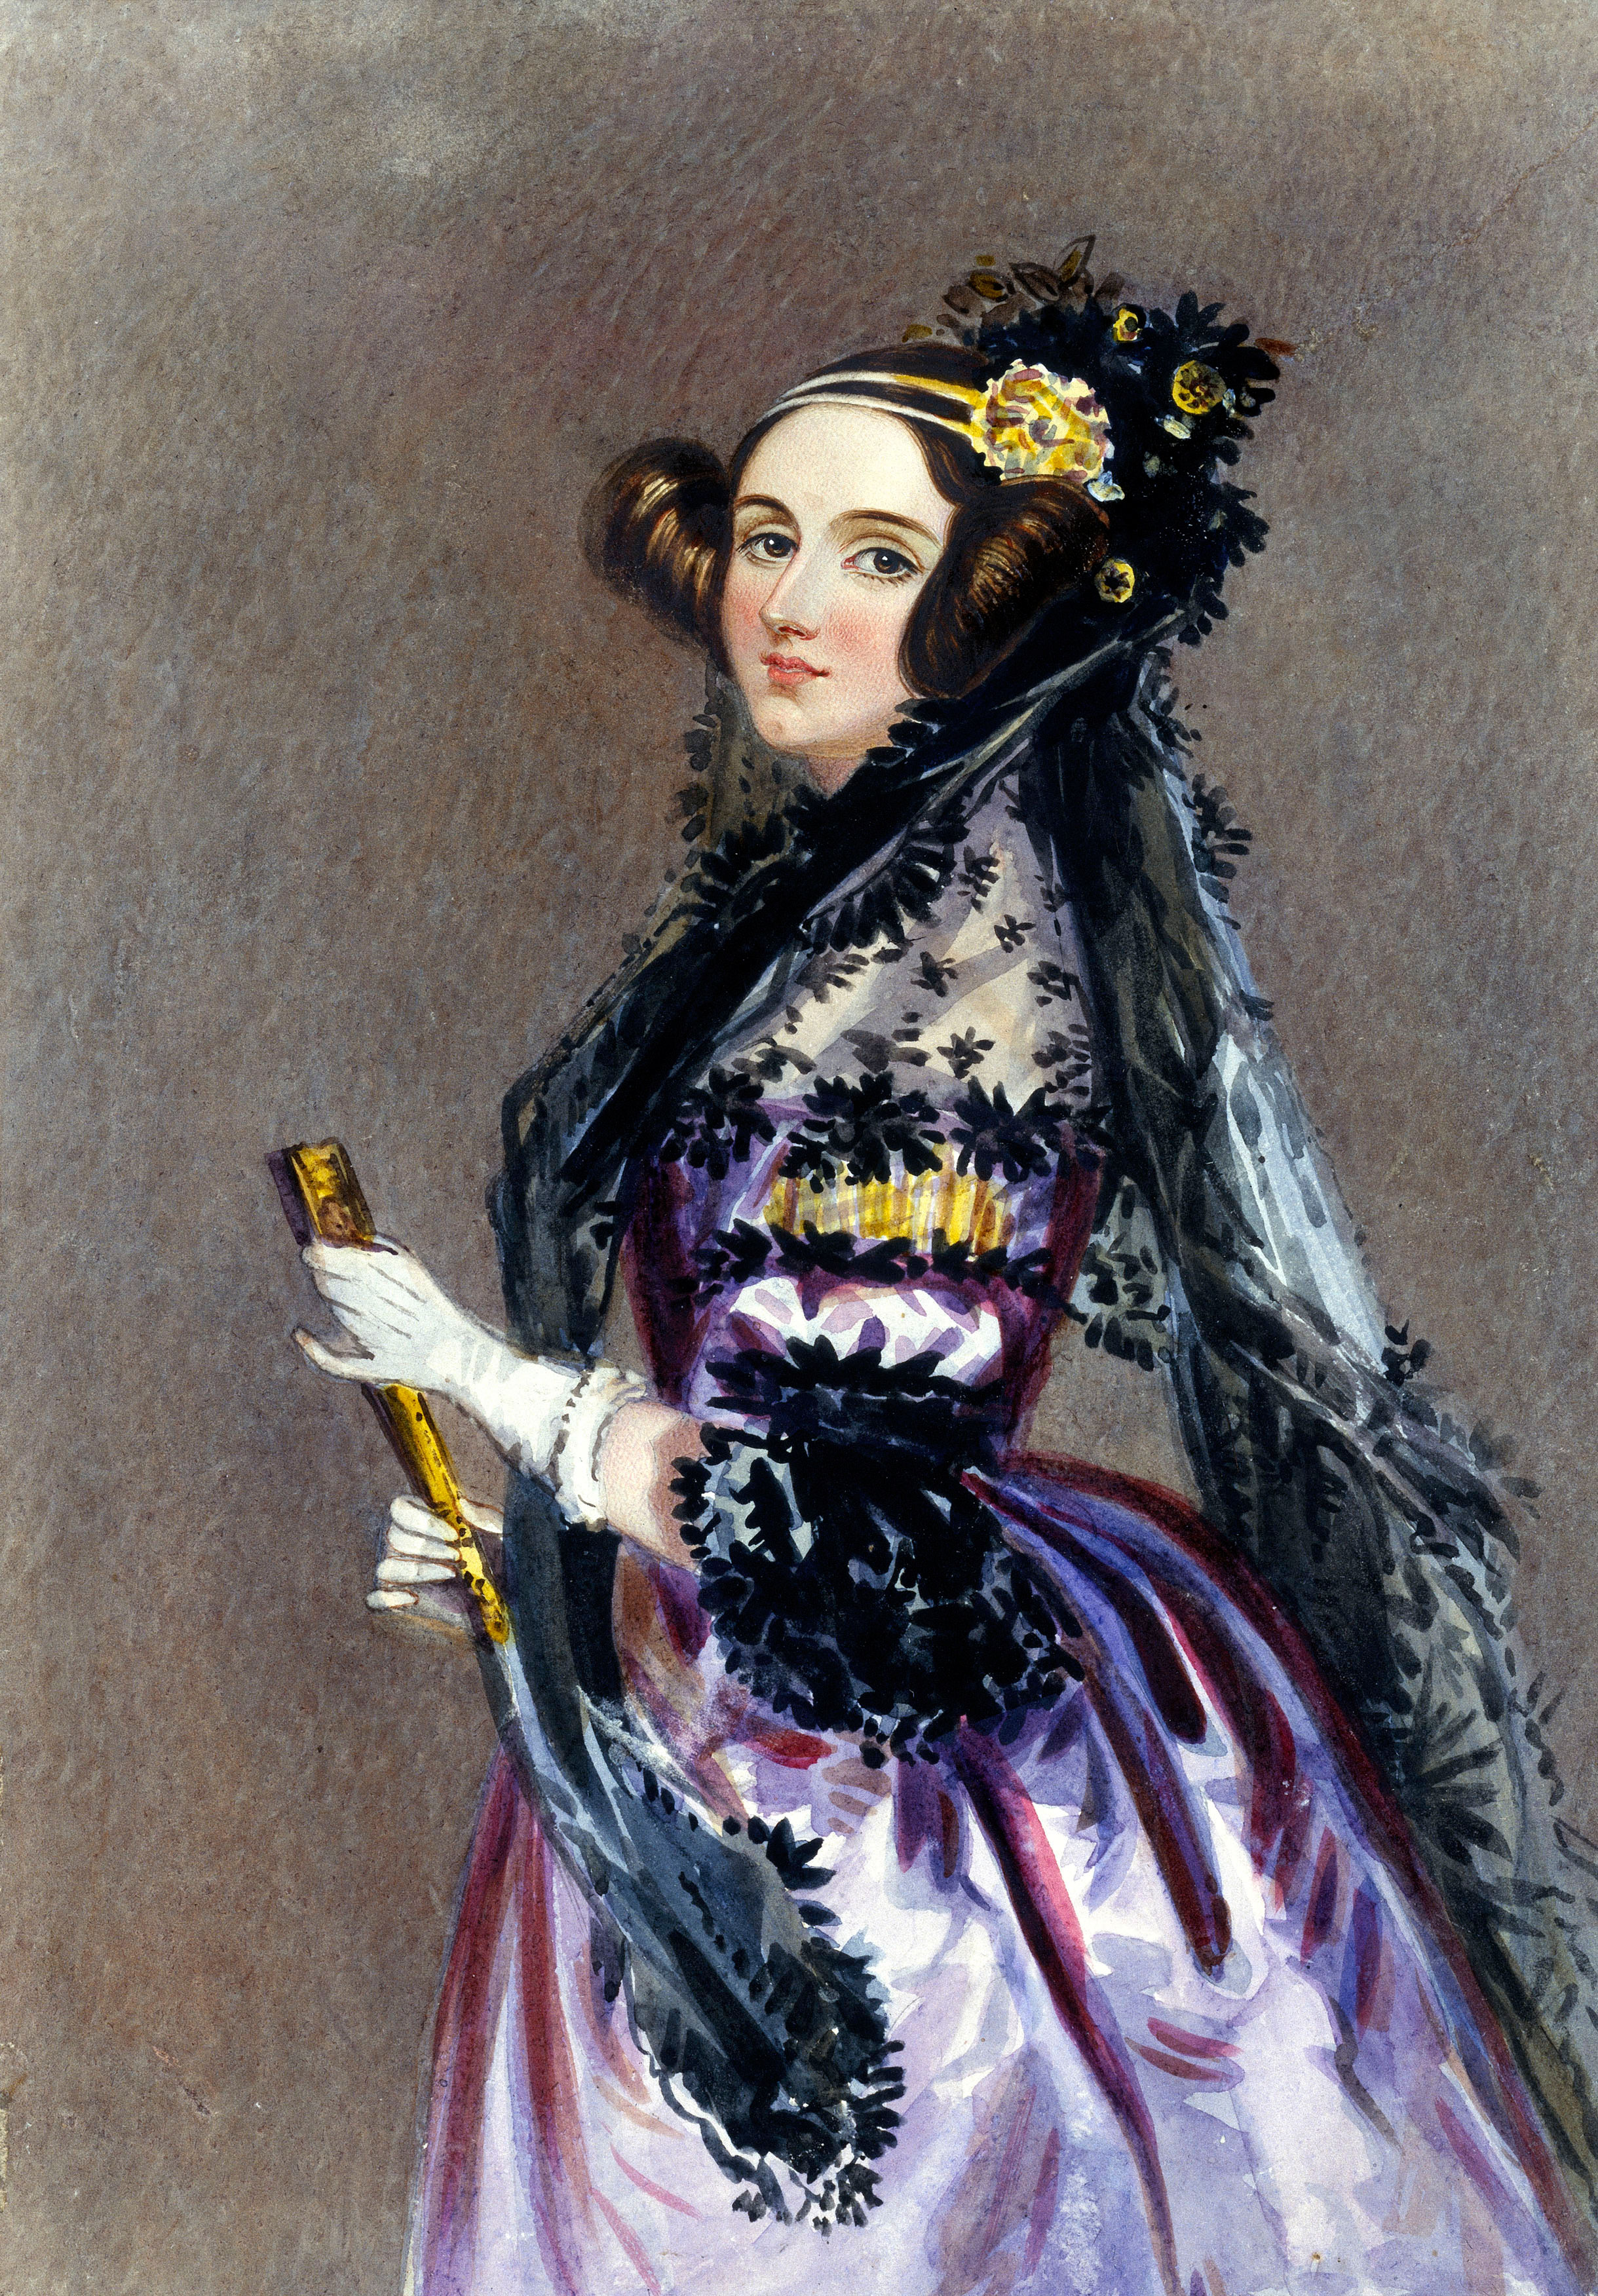
\includegraphics[width=0.4\linewidth]{graphics/Ada_Lovelace_portrait.jpg}
\caption{The portrait of Ada Lovelace.}
\label{fig:ada}
\end{figure}
First, we need to enclose the \texttt{\textbackslash includegraphics} command within a \verb|figure| environment. The \verb|ht!| option indicates that priority is given to put the figure structure exactly in the place where the code is inserted (\verb|h|: here), or at the top of a page (\verb|t|). The \verb|width| option enforces the width of the image to the input value (and similarly there are \verb|height| and \verb|scale|). The \verb|caption| command unsurprisingly generates the caption, while the \verb|label| command works as it is in math mode and allows us to reference it by writing \texttt{\textbackslash ref\{fig:ada\}}.

\paragraph{subcaption}
We can construct a set of subfigures within an overarching figure by utilizing the \verb|subcaption| package and \verb|subfigure| groups. To illustrate, the following code is deployed to generate Figure \ref{fig:TC1}: 
\begin{lstlisting}
\begin{figure}[ht!]
\centering
\begin{subfigure}[b]{0.45\textwidth}
\centering
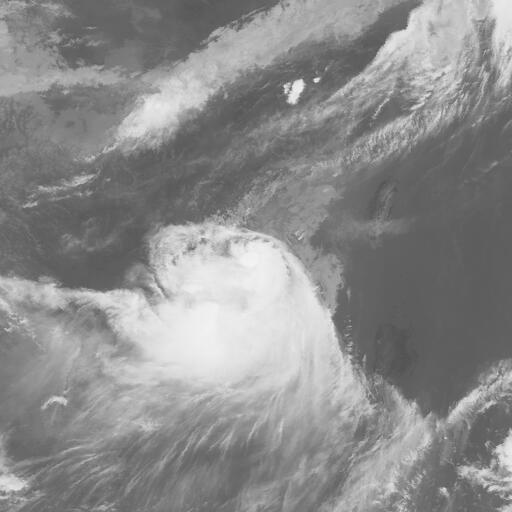
\includegraphics[width=0.8\linewidth]{graphics/MTS108082203.200812.jpg}
\caption{Typhoon Nuri (2008).}
\end{subfigure}
\begin{subfigure}[b]{0.45\textwidth}
\centering
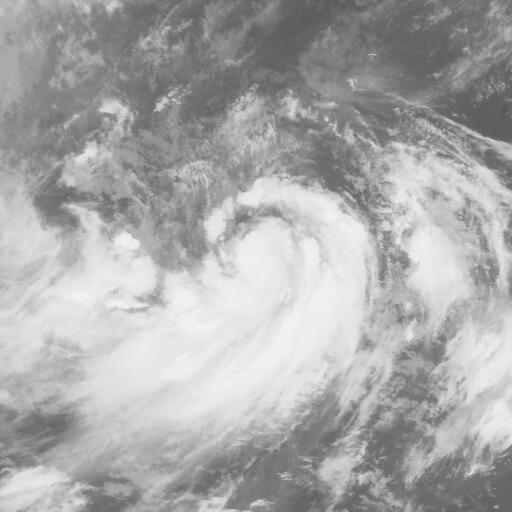
\includegraphics[width=0.8\linewidth]{graphics/MTS212072303.201208.jpg}
\caption{Typhoon Vicente (2012).}
\end{subfigure}
\caption{The infrared satellite images of various Tropical Cyclones affecting Hong Kong.}
\label{fig:TC1}
\end{figure}   
\end{lstlisting}
The \verb|b| option sets the vertical alignment of \verb|subfigure| at the bottom.

\begin{figure}[ht!]
\centering
\begin{subfigure}[b]{0.45\textwidth}
\centering
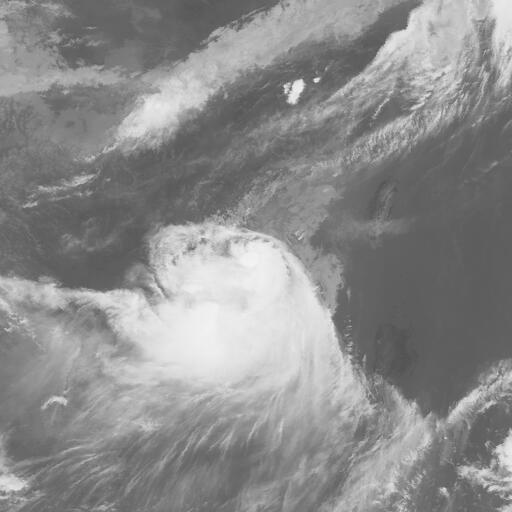
\includegraphics[width=0.8\linewidth]{graphics/MTS108082203.200812.jpg}
\caption{Typhoon Nuri (2008).}
\end{subfigure}
\begin{subfigure}[b]{0.45\textwidth}
\centering
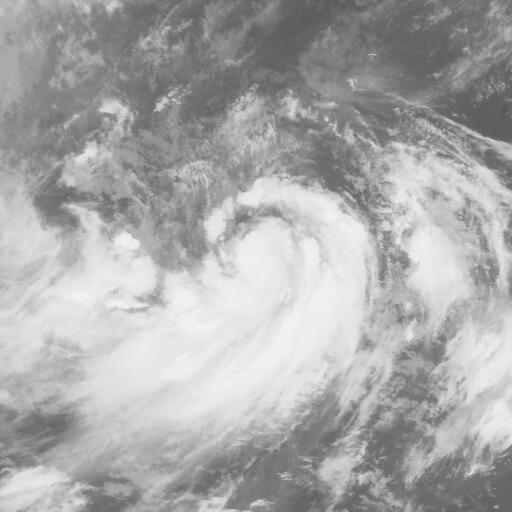
\includegraphics[width=0.8\linewidth]{graphics/MTS212072303.201208.jpg}
\caption{Typhoon Vicente (2012).}
\end{subfigure}
\caption{The infrared satellite images of various Tropical Cyclones affecting Hong Kong. (Source: \href{https://agora.ex.nii.ac.jp/digital-typhoon/index.html.en}{Digital Typhoon})}
\label{fig:TC1}
\end{figure}

\paragraph{ContinuedFloat} To make a longer figure of subfigures that spans multiple pages, we can simply arrange them into separate \verb|figure| environments and call the \texttt{\textbackslash ContinuedFloat} command in all the subsequent \verb|figure| groups. Continuing from the last example, we may have
\begin{lstlisting}
\begin{figure}[hb!]
\ContinuedFloat % here!
\caption{(Cont.) The infrared satellite images of various Tropical Cyclones affecting Hong Kong.}
\centering
\begin{subfigure}[b]{0.45\textwidth}
...
\caption{Typhoon Haima (2016).}
\end{subfigure}
...
\begin{subfigure}[b]{0.45\textwidth}
...
\caption{Typhoon Saola (2023).}
\end{subfigure}
\end{figure}    
\end{lstlisting}
producing
\begin{figure}[hb!]
\ContinuedFloat
\caption{(Cont.) The infrared satellite images of various Tropical Cyclones affecting Hong Kong.}
\centering
\begin{subfigure}[b]{0.45\textwidth}
\centering
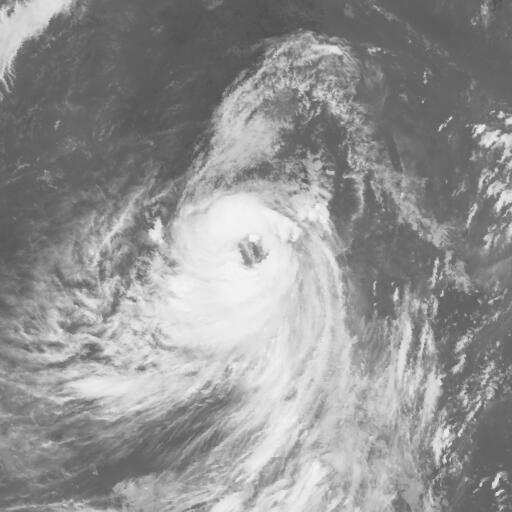
\includegraphics[width=0.8\linewidth]{graphics/HMW816080103.201604.jpg}
\caption{Typhoon Haima (2016).}
\end{subfigure}
\begin{subfigure}[b]{0.45\textwidth}
\centering
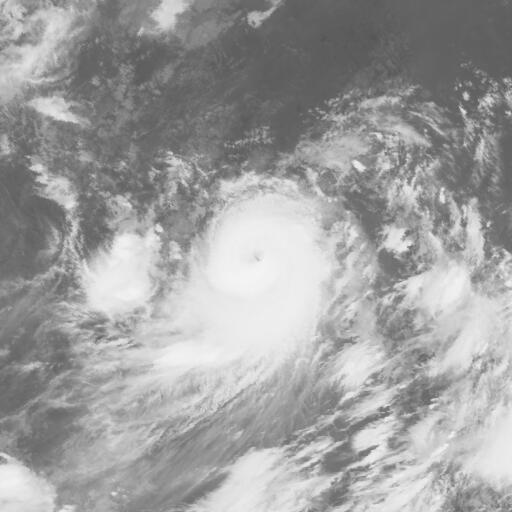
\includegraphics[width=0.8\linewidth]{graphics/HMW817082303.201713.jpg}
\caption{Typhoon Hato (2017).}
\end{subfigure}
\begin{subfigure}[b]{0.45\textwidth}
\centering
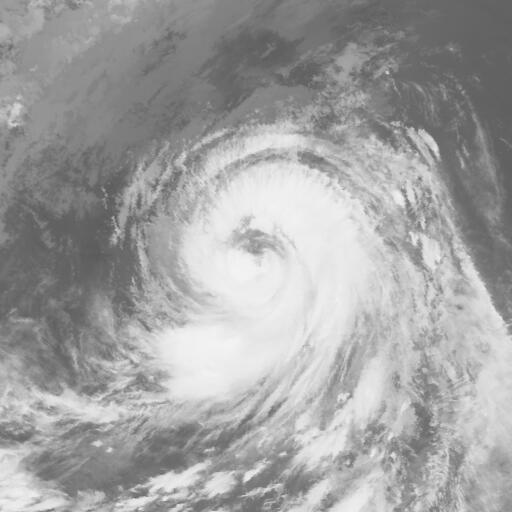
\includegraphics[width=0.8\linewidth]{graphics/HMW818091603.201822.jpg}
\caption{Typhoon Mangkhut (2018).}
\end{subfigure}
\begin{subfigure}[b]{0.45\textwidth}
\centering
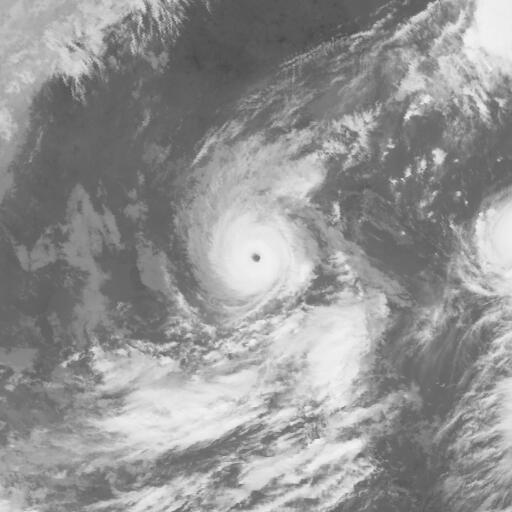
\includegraphics[width=0.8\linewidth]{graphics/HMW923090103.202309.jpg}
\caption{Typhoon Saola (2023).}
\end{subfigure}
\end{figure}

\subsection{Tables}

\paragraph{table, tabularx}
Just like embedding figures, building a table requires us to place the content inside the corresponding \verb|table| environment. While it is possible to use the native \verb|tabular| class for the actual table itself, a more powerful version is provided by the \verb|tabularx| package and its class that bears the same name. This is demonstrated via Table \ref{tab:armyunits} thereafter, which is generated by
\begin{lstlisting}
\begin{table}[ht!]
\centering
\begin{tabularx}{\textwidth}{|l|p{0.55\textwidth}|>{\raggedleft}X|>{\raggedleft\arraybackslash}X|}
\hline
Unit & Description & Attack & Defense \\
\hline
Infantry & The most basic unit and backbone of any army, all-around abilities with a cheap cost. & 20 & 25 \\
\hline
Cavalry & The shock unit in an army with very strong power. & 40 & 30 \\
\hline
Artillery & The support unit that provides bombardment support from far away. & 30 & 5 \\
\hline
\end{tabularx}
\caption{The unit statistics table for a hypothetical game.}
\label{tab:armyunits}
\end{table}
\end{lstlisting}
\begin{table}[ht!]
\centering
\begin{tabularx}{\textwidth}{|l|p{0.55\textwidth}|>{\raggedleft}X|>{\raggedleft\arraybackslash}X|}
\hline
Unit & Description & Attack & Defense \\
\hline
Infantry & The most basic unit and backbone of any army, all-around abilities with a cheap cost. & 20 & 25 \\
\hline
Cavalry & The shock unit in an army with very strong power. & 40 & 30 \\
\hline
Artillery & The support unit that provides bombardment support from far away. & 30 & 5 \\
\hline
\end{tabularx}
\caption{The unit statistics table for a hypothetical game.}
\label{tab:armyunits}
\end{table}
The \verb|ht!| option, \verb|caption|, and \verb|label| work exactly as the figure counterpart. For the \verb|tabularx| group, the first argument indicates the width of the entire table, set to \texttt{\textbackslash textwidth} here. The second argument \texttt{\{|l|p\{0.55\textbackslash textwidth\}|\allowbreak >\{\textbackslash raggedleft\}X|>\{\textbackslash raggedleft\textbackslash arraybackslash\}X|\}} indicates the justification of the columns: the first column is left-aligned (\verb|l|, similarly we have \verb|c| and \verb|r|) and its size will fit the text; the second column (\verb|p|) forces a width of $0.55$ times \texttt{\textbackslash textwidth}; the remaining width is distributed evenly to last two columns (\verb|X|). The part of \texttt{>\{\textbackslash raggedleft\}} is applied to the \verb|X| columns, making them right-aligned.\footnote{\texttt{\textbackslash arraybackslash} is needed in the last column, see \href{https://tex.stackexchange.com/questions/372464/last-tabularx-column-raggedright-with-memoir}{\TeX{} StackExchange 372464}.} Finally, \texttt{|} and \texttt{\textbackslash hline} produce vertical/horiztonal separating lines; \texttt{\&} slices between the columns and \texttt{\textbackslash\textbackslash} marks the end of a row.

Also, note that \texttt{\textbackslash ContinuedFloat} can also be applied to \texttt{table}.

\paragraph{captionbeside} It is also possible to arrange the table so that the caption appears to the side of it. This is done by stacking the \verb|captionbeside| environment provided by KOMA-script. For example, the code
\begin{lstlisting}
\begin{table}[ht]
\begin{captionbeside}{This caption appears to the left of the Fibonacci numbers table.}[l][\textwidth]{
\adjustbox{valign=t}{
    \begin{tabularx}{0.4\textwidth}{|X|X|}
    \hline
    $n$ & $F_n$ \\
    \hline 
    $1$ & $1$ \\
    \hline 
    $2$ & $1$ \\
    \hline 
    $3$ & $2$ \\
    \hline 
    $4$ & $3$ \\
    \hline
    $5$ & $5$ \\
    \hline
    $6$ & $8$ \\
    \hline
    \end{tabularx}}
}
\end{captionbeside}
\label{tab:fib}
\end{table}    
\end{lstlisting}
produces Table \ref{tab:fib} below.

\begin{table}[ht]
\begin{captionbeside}{This caption appears to the left of the Fibonacci numbers table.}[l][\textwidth]{\adjustbox{valign=t}{\begin{tabularx}{0.4\textwidth}{|X|X|}
\hline
$n$ & $F_n$ \\
\hline 
$1$ & $1$ \\
\hline 
$2$ & $1$ \\
\hline 
$3$ & $2$ \\
\hline 
$4$ & $3$ \\
\hline
$5$ & $5$ \\
\hline
$6$ & $8$ \\
\hline
\end{tabularx}}}
\end{captionbeside}
\label{tab:fib}
\end{table}
We fill the caption in the first argument, followed by the relative position of the caption (\verb|l|: left) and the full width of the structure, finally with the actual \verb|tabularx| object. We also have to additionally load the \verb|adjustbox| package and use the corresponding command to tell the table to align itself at the top (\verb|valign=t|). This also requires us to first set the \texttt{\textbackslash KOMAoptions} to take \verb|captions=besidetop| (likewise we have \verb|captions=besidebottom| and more).

\paragraph{Shared Numbering between Figures and Tables}
Sometimes we may want to share the numbering between \textit{floats} (including figures, tables, and so on). This is done by the following patch that can be inserted into the preamble:
\begin{lstlisting}
\makeatletter
\let\c@table\c@figure
\let\ftype@table\ftype@figure
\makeatother
\end{lstlisting}
This involves the primitive \TeX{} functions, so we will not discuss them there. For more information, read \href{https://stackoverflow.com/questions/3865036/using-a-single-count-for-figures-and-tables-in-latex}{StackOverflow 3865036}, and \href{https://tex.stackexchange.com/questions/8351/what-do-makeatletter-and-makeatother-do}{\TeX{} StackExchange 8351} for what the \texttt{\textbackslash makeatletter} and \texttt{\textbackslash makeatother} commands do.

\begin{exercisebox}
\begin{Exercise}
Try to import and load your favorite image into the document. 
\end{Exercise}
\begin{Exercise}
Recreate any one of the tables in Chapter \ref{chap:maths}.
\end{Exercise}
\end{exercisebox}

\section{Minipages and Multiple Columns}

\paragraph{minipage}
Sometimes we may want to partition the content into smaller blocks that are embedded within the current page, and can be placed or ordered (e.g.\ parallel) in the way we want. The \verb|minipage| environment basically acts like a more versatile version of a \verb|parbox| environment and serves this purpose. For example, something like
\begin{lstlisting}
yields \par
\begin{center}
\begin{minipage}[b]{0.48\textwidth}
\lipsum[6]
\end{minipage}
\hfill
\begin{minipage}[b]{0.48\textwidth}
\lipsum[7]
\end{minipage}    
\end{center}      
\end{lstlisting}
yields \par
\begin{center}
\begin{minipage}[b]{0.48\textwidth}
\lipsum[6]
\end{minipage}
\hfill
\begin{minipage}[b]{0.48\textwidth}
\lipsum[7]
\end{minipage}    
\end{center}
The \verb|[b]| option indicates the baseline is set at the bottom, and hence the two blocks will be bottom-aligned, provided that their width is fixed to $0.48$ times \texttt{\textbackslash textwidth} and thus they fit in the main text area.

\paragraph{parcolumns} The \verb|parcolumns| package can also achieve the above effect and is more specialized for typesetting different pieces in two or more parallel columns. It also supports page breaks. Using the same example, we can write
\begin{lstlisting}
\begin{parcolumns}{2}
\colchunk[1]{\lipsum[6]}
\colchunk[2]{\lipsum[7]}
\colplacechunks
\colchunk[1]{\lipsum[8]}
\colchunk[2]{\lipsum[9]}
\end{parcolumns}
\end{lstlisting}
to get\\
\begin{parcolumns}{2}
\colchunk[1]{\lipsum[6]}
\colchunk[2]{\lipsum[7]}
\colplacechunks
\colchunk[1]{\lipsum[8]}
\colchunk[2]{\lipsum[9]}
\end{parcolumns}
where the first argument of the environment clearly indicates the number of columns and the \texttt{\textbackslash colplacechunks} command releases the loaded \texttt{\textbackslash colchunk[<col\allowbreak\_no.>]} and goes to the next paragraph.

\paragraph{multicol} A task closely related to what \verb|parcolumns| does above is to typeset a single, continuous stream of text along multiple columns, like in many academic papers. The \texttt{multicol} package is designed for this and will carry out the automatic splitting. For example, by encapsulating the text inside the \verb|multicols| environment as
\begin{lstlisting}
\begin{multicols}{2}
Zhuge Liang (born 181, Yangdu [now Yinan, Shandong province], China--died August 234, Wuzhangyuan [now in Shaanxi province], China) was a celebrated adviser to Liu Bei, founder of the Shu-Han dynasty (221--263/264).
...
A mechanical and mathematical genius, Zhuge is credited with inventing a bow for shooting several arrows at once and with perfecting the Eight Dispositions, a series of military tactics. In the Sanguozhi yanyi (Romance of the Three Kingdoms), the great 14th-century historical novel, Zhuge is one of the main characters; he is portrayed as being able to control the wind and foretell the future.
\end{multicols}
\end{lstlisting}
(again with the number of columns indicated in the first argument) we may acquire the following layout:
\begin{multicols}{2}
Zhuge Liang (born 181, Yangdu [now Yinan, Shandong province], China--died August 234, Wuzhangyuan [now in Shaanxi province], China) was a celebrated adviser to Liu Bei, founder of the Shu-Han dynasty (221--263/264).

Quick Facts: \\
Wade-Giles romanization: Chu-ko Liang \\
Courtesy name: Kongming \\
Born: 181, Yangdu [now Yinan, Shandong province], China \\
Died: August 234, Wuzhangyuan [now in Shaanxi province], China (aged 53)

Zhuge, to whom supernatural powers often are ascribed, has been a favoured character of many Chinese plays and stories. Legend states that Liu Bei, then a minor military figure, heard of Zhuge Liang’s great wisdom and came three times to the wilderness retreat to which Zhuge had retired to seek him out as an adviser. It is known that Zhuge helped Liu organize a large army and found a dynasty. Liu was so impressed with Zhuge’s wisdom that on his deathbed Liu urged his son to depend on Zhuge’s advice and urged Zhuge to ascend the throne himself if the prince were unable to rule. Some historical accounts indicate that Zhuge died from illness while leading a military campaign in 234.

A mechanical and mathematical genius, Zhuge is credited with inventing a bow for shooting several arrows at once and with perfecting the Eight Dispositions, a series of military tactics. In the Sanguozhi yanyi (Romance of the Three Kingdoms), the great 14th-century historical novel, Zhuge is one of the main characters; he is portrayed as being able to control the wind and foretell the future. (Source: Encyclopaedia Britannica)
\end{multicols}


\paragraph{twocolumn} We can also pass the \verb|twocolumn=true| option to \texttt{\textbackslash KOMAoptions} to demand the entire book to be formatted in two columns globally. However, note that it will greatly mess up the layout of this book. (The decision to adopt such a format should be made at an early time!)